\section{Upper limits at 90\% confidence levels}

Figures~\ref{S6_H1_UL} and~\ref{S6_L1_UL} show tentative ULs that, in the final analysis, correspond to approximately 90\% confidence for random polarization.
The 90\% confidence level requires a correction factor of $h_0 \times \left(1+0.8 \right) \left[\cos \iota \textup{ factor} \right]$.
These figures also illustrate the most sensitive part of the LIGO spectrum.

\begin{figure}
\begin{center}
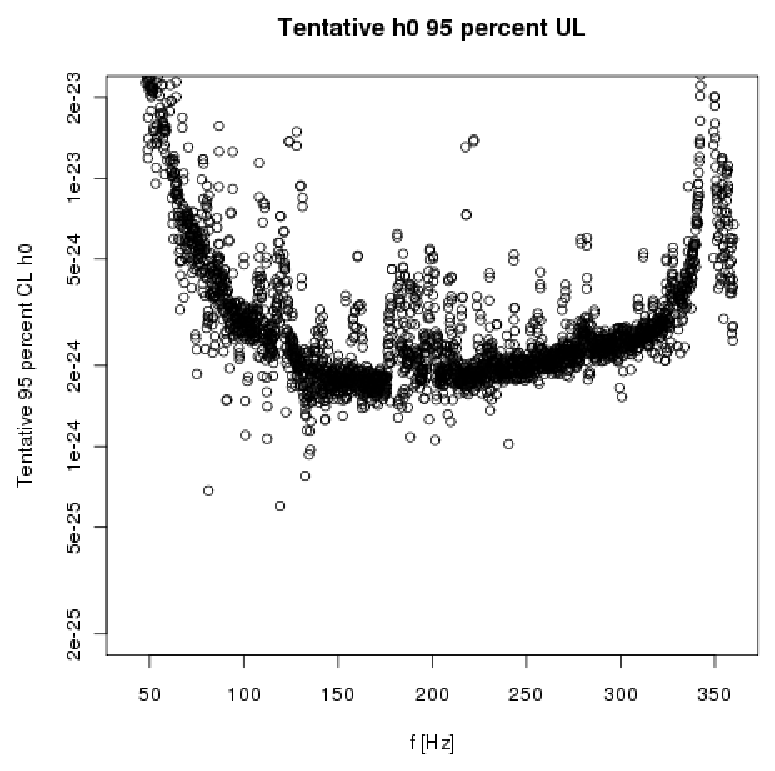
\includegraphics[width=0.68\paperwidth,height=0.48\paperheight]{plots/h0FullUL95logGuess-H1.eps}
\caption{
H1: loudest $h_0 \times \left( 1 + 0.8 \right) \times \left[\cos \iota \textup{ factor}\right]$ in 0.1 Hz bands. 
The `Tentative $h_0$ 95 percent UL' statement was later revised; the 95\% confidence level is higher by $2.0/1.8$.
This plot shown corresponds to about 90\% confidence in random polarization ULs in the final analysis.}
\label{S6_H1_UL}
\end{center}
\end{figure}

\begin{figure}
\begin{center}
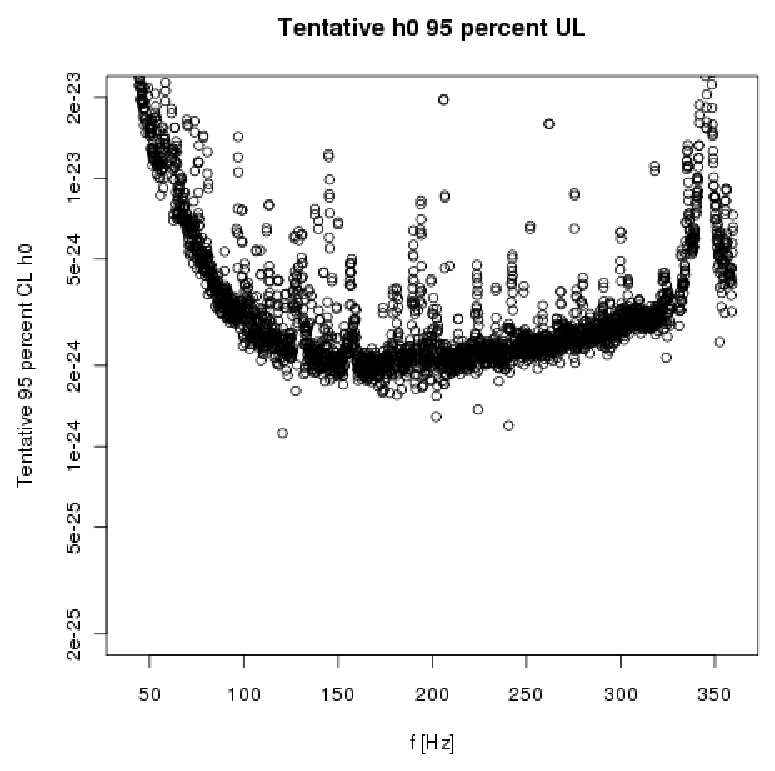
\includegraphics[width=0.68\paperwidth,height=0.48\paperheight]{plots/h0FullUL95logGuess-L1.eps}
\caption{
L1: loudest $h_0 \times \left( 1 + 0.8 \right) \times \left[\cos \iota \textup{ factor}\right]$ in 0.1 Hz bands. 
The `Tentative $h_0$ 95 percent UL' statement was later revised; the 95\% confidence level is higher by $2.0/1.8$.
This plot shown corresponds to about 90\% confidence in random polarization ULs in the final analysis.}
\label{S6_L1_UL}
\end{center}
\end{figure}


\section{Preliminary high frequency outliers}

The production analysis of Scorpius X-1 data in Chapter~\ref{chap6} yielded the following lists of Stage I outliers for follow-up, detailed in Tables~\ref{ScoX1S6outlierTableHF1} to~\ref{ScoX1S6outlierTableHF3}, covering coincident outliers (present in both intereferometers) between 360 and 2040 Hz.
These and the outliers in Table~\ref{ScoX1S6outlierTable} are planned to be followed-up with run-averaged spectra and strain histograms, and their relative values in H1 and L1 will be compared.
When finished, we will have an indication whether these outliers are artifacts, as expected, or could be signals from Scorpius X-1.

\begin{table}
\begin{center}
\begin{tabular}{r r l}
Outlier Number & Frequency (Hz) & Explanation \\
\hline
23 & 360.01  & -- \\
24 & 360.10 & -- \\
25 & 361.47 & -- \\
26 & 375.37 & -- \\
27 & 383.18 & -- \\
28 & 400.10 & -- \\
29 & 403.77 & -- \\
30 & 404.80 & -- \\
31 & 419.79 & -- \\
32 & 419.89 & -- \\
33 & 420.00 & -- \\
34 & 420.10 & -- \\
35 & 420.20 & -- \\
36 & 435.25 & -- \\
37 & 440.10 & -- \\
38 & 448.08 & -- \\
39 & 450.95 & -- \\
40 & 468.10 & -- \\
41 & 479.88 & -- \\
42 & 479.92 & -- \\
43 & 479.95 & -- \\
44 & 480.01 & -- \\
45 & 480.10 & -- \\
46 & 482.21 & -- \\
47 & 500.05 & -- \\
48 & 539.95 & -- \\
49 & 540.00 & -- \\
50 & 540.10 & -- \\
51 & 551.85 & -- \\
52 & 552.02 & -- \\
53 & 568.10 & -- \\
54 & 570.35 & -- \\
55 & 599.78 & -- \\
56 & 599.89 & -- \\
57 & 600.00 & -- \\
58 & 600.06 & -- \\
59 & 646.52 & -- \\
60 & 656.64 & -- \\
61 & 691.00 & -- \\
62 & 691.07 & -- \\
63 & 691.15 & -- \\
64 & 692.14 & -- \\
65 & 719.78 & -- \\
66 & 719.89 & -- \\
67 & 719.97 & -- \\
68 & 720.03 & -- \\
69 & 770.23 & -- \\
70 & 839.99 & -- \\
71 & 870.00 & -- \\
\end{tabular}
\caption{List of Scorpius X-1 outliers in stage I of the search of S6 data. This list covers 360 to 900 Hz.}
\label{ScoX1S6outlierTableHF1}
\end{center}
\end{table}

\begin{table}
\begin{center}
\begin{tabular}{r r l}
Outlier Number & Frequency (Hz) & Explanation \\
\hline
72 & 908.93 & -- \\
73 & 942.74 & -- \\
74 & 957.69 & -- \\
75 & 963.21 & -- \\
76 & 1022.97 & -- \\
77 & 1033.98 & -- \\
78 & 1091.47 & -- \\
79 & 1098.21 & -- \\
80 & 1147.69 & -- \\
81 & 1166.13 & -- \\
82 & 1166.20 & -- \\
83 & 1171.08 & -- \\
84 & 1190.61 & -- \\
85 & 1216.10 & -- \\
86 & 1305.99 & -- \\
87 & 1306.12 & -- \\
88 & 1306.36 & -- \\
89 & 1306.47 & -- \\
90 & 1306.66 & -- \\
91 & 1306.97 & -- \\
92 & 1307.06 & -- \\
93 & 1312.45 & -- \\
94 & 1318.69 & -- \\
95 & 1374.10 & -- \\
96 & 1375.81 & -- \\
97 & 1397.90 & -- \\
98 & 1398.22 & -- \\
99 & 1489.21 & -- \\
100 & 1495.19 & -- \\
101 & 1495.29 & -- \\
102 & 1495.50 & -- \\
103 & 1495.94 & -- \\
104 & 1496.00 & -- \\
105 & 1505.59 & -- \\
106 & 1506.02 & -- \\
107 & 1514.16 & -- \\
108 & 1563.03 & -- \\
109 & 1574.28 & -- \\
110 & 1578.44 & -- \\
111 & 1600.32 & -- \\
112 & 1607.70 & -- \\
113 & 1607.90 & -- \\
114 & 1608.00 & -- \\
115 & 1608.08 & -- \\
116 & 1611.51 & -- \\
117 & 1627.74 & -- \\
\end{tabular}
\caption{List of Scorpius X-1 outliers in stage I of the search of S6 data. This list covers 900 to 1700 Hz.}
\label{ScoX1S6outlierTableHF2}
\end{center}
\end{table}

\begin{table}
\begin{center}
\begin{tabular}{r r l}
Outlier Number & Frequency (Hz) & Explanation \\
\hline
118 & 1719.26 & -- \\
119 & 1719.40 & -- \\
120 & 1738.20 & -- \\
121 & 1738.63 & -- \\
122 & 1738.76 & -- \\
123 & 1738.92 & -- \\
124 & 1824.02 & -- \\
125 & 1842.91 & -- \\
126 & 1920.08 & -- \\
127 & 1940.69 & -- \\
128 & 1940.81 & -- \\
129 & 1976.25 & -- \\
130 & 2005.58 & -- \\
131 & 2007.77 & -- \\
\end{tabular}
\caption{List of Scorpius X-1 outliers in stage I of the search of S6 data. This list covers 1700 to 2040 Hz.}
\label{ScoX1S6outlierTableHF3}
\end{center}
\end{table}



